\chapter{Theoretical Framework}\label{ch:theory}

\section{Binary floating-point spacing}
A normal binary floating-point number of precision $p$ can be written
\begin{equation}\label{eq:float}
 y=M\,2^{E-p+1},\qquad 2^{p-1}\le M<2^p,\quad M\in\mathbb{Z},
\end{equation}
where $E=\lfloor\log_2 y\rfloor$ is the binade exponent. If $y\in[2^E,2^{E+1})$, the upward spacing throughout the interior of that binade is
\begin{equation}\label{eq:ulp}
 u=\ulp(y)=2^{E-p+1}.
\end{equation}
The spacing is constant within each binade and doubles at the next power of two. For binary64, the transition from $u=1$ to $u=2$ occurs at $y=2^{53}$; when $y\approx x^{10}$, this corresponds to $x\approx2^{53/10}\approx39.3966$. In binary32, the analogous transition is at $x\approx2^{24/10}\approx5.2780$.

\begin{figure}[htbp]
\centering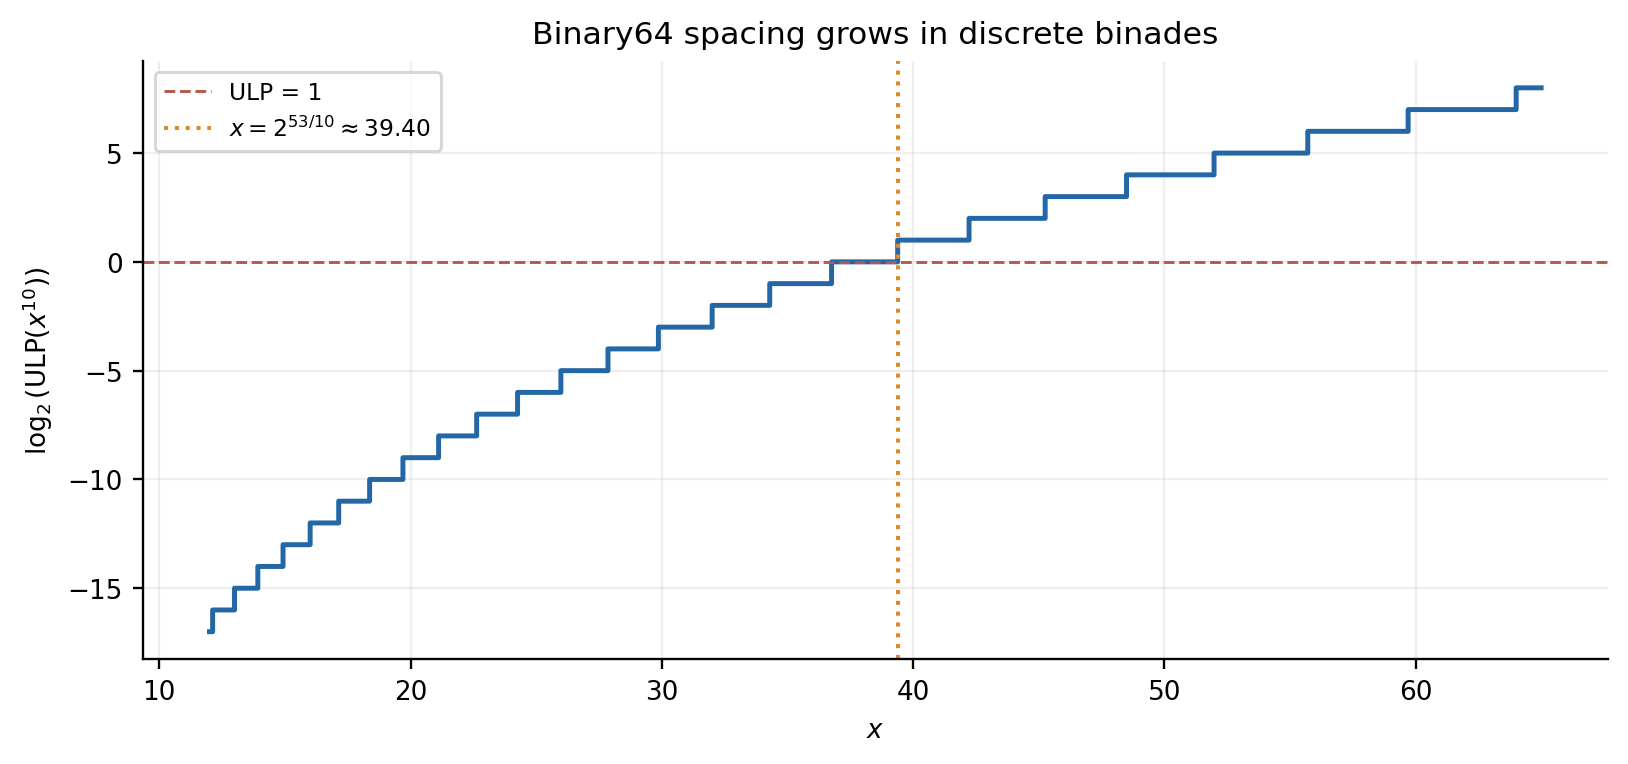
\includegraphics[width=.91\textwidth]{figs/01_ulp_staircase.png}
\caption{Reconstructed binary64 ULP staircase for $x^{10}$. The dashed line marks $u=1$, and the dotted line marks the $u=2$ transition.}\label{fig:ulp}
\end{figure}

\section{The computed function and exact final subtraction}
Let
\begin{equation}\label{eq:fn}
 y=\fl(x^{10}),\qquad s=\fl(y+c),\qquad f(x;c)=\fl(s-y).
\end{equation}
A central fact is that the subtraction in Equation~\eqref{eq:fn} need not introduce an additional error. Under $y\ge c>0$ and normal finite arithmetic, $s$ is sufficiently close to $y$ for the subtraction to be exact by Sterbenz's lemma (which states that $a-b$ is exactly representable when two floating-point operands satisfy $b/2\le a\le2b$ under the usual exponent-range hypotheses) \cite{sterbenz1974floating,higham2002accuracy}. Thus $f=s-y$ and the local error arises from the rounded addition.

Write the positive stored increment in lowest binary terms as
\begin{equation}\label{eq:nu}
 c=m2^{\nu},\qquad m\text{ a positive odd integer},\quad
 \lambda=\lfloor\log_2 c\rfloor.
\end{equation}
Here $\nu=\nu(c)$ is the exponent of the least significant nonzero bit in the exact stored value of $c$. This is meaningful even when the user typed a non-dyadic decimal: the stored binary32 or binary64 number is always dyadic.

\section{Nearest-grid rule and ties}
\begin{proposition}[Binade-wise rounding model]\label{prop:grid}
Assume round-to-nearest, ties-to-even; $y\ge c>0$; reuse of the same stored $y$; and $y+c<2^{E+1}$, so the exact sum remains in the same binade. Set $u=2^{E-p+1}$, $M=y/u\in\mathbb{Z}$, and $q=c/u$. Then
\begin{equation}\label{eq:grid}
 f(x;c)=u\,k,\quad k=\begin{cases}
 q, & q\in\mathbb{Z},\\
 \lfloor q+\tfrac12\rfloor,&q\notin\mathbb{Z}+\tfrac12,\\
 \text{the integer in }\{\lfloor q\rfloor,\lceil q\rceil\}
 \text{ for which }M+k\text{ is even}, &q\in\mathbb{Z}+\tfrac12.
 \end{cases}
\end{equation}
\end{proposition}
\begin{proof}
The stored $y=Mu$ is a point on the binade's representable grid. Rounding $y+c=u(M+q)$ to nearest selects $s=u(M+k)$, with ties resolved by even $M+k$. Sterbenz's lemma makes the final subtraction exact, yielding $f=s-y=uk$.
\end{proof}

In particular, all ties depend on the parity of the stored significand $M$, not only on the magnitude of $c$. For example, at $x=40$ in binary64, $y=40^{10}=10{,}485{,}760{,}000{,}000{,}000$ is exactly representable, $u=2$, and $M$ is even. Thus $c=1$ gives $f=0$, $c=3$ gives $f=4$, and $c=5$ gives $f=4$. A neighboring stored $y$ with odd $M$ can select the other side of a tie.

\section{Thresholds and the width of the inexact region}
\begin{proposition}[Transition binades]\label{prop:thresholds}
Under the hypotheses of Proposition~\ref{prop:grid}, let
\begin{equation}\label{eq:bounds}
 E_1=p+\nu,\qquad E_2=p+\lambda,\qquad
 L=E_2-E_1+1=\lambda-\nu+1.
\end{equation}
Below $E_1$, the grid resolves $c$ exactly. At $E_1$, the increment lies exactly halfway between two grid points and the result alternates between $c-u/2$ and $c+u/2$ according to parity. In subsequent binades through $E_2$, the rounded increment is a binade-dependent multiple of $u$; above $E_2$ it is zero. Consequently, in terms of $x$ the predicted transition interval is approximately
\begin{equation}\label{eq:xthreshold}
 x_1=2^{(p+\nu)/10},\qquad
 x_2=2^{(p+1+\lambda)/10},\qquad
 \frac{x_2}{x_1}=2^{L/10}.
\end{equation}
These are thresholds in the exponent of the \emph{computed} $y$; their numerical $x$ locations may shift slightly because $y=\fl(x^{10})$ and because of finite input sampling.
\end{proposition}
\begin{proof}
If $u\le2^{\nu}$, the power-of-two grid spacing divides $c=m2^{\nu}$, so $c/u$ is an integer and Equation~\eqref{eq:grid} returns $c$. The first larger spacing is $u=2^{\nu+1}$, where $q=m/2$ is a half-integer. For still larger powers of two, $q$ is neither integral nor halfway between consecutive integers. The rounded result becomes identically zero once $u>2c$, i.e., for exponents $E>p+\lambda$. The number of potentially inexact binades is therefore $L=(p+\lambda)-(p+\nu)+1$. The conversion from exponents of $y\approx x^{10}$ produces Equation~\eqref{eq:xthreshold}. If $c$ is itself a power of two, the final tie binade can yield either zero or $2c$; the fully absorbed regime starts in the following binade.
\end{proof}

The integer $L$ is the binary bit length of the odd significand $m$. For $c=2^j$, $L=1$. For positive odd integers, $\nu=0$ and $L=\lfloor\log_2 c\rfloor+1$. For typical stored approximations to non-dyadic fractions, $L$ is close to the full precision $p$.

\section{Error measured in ULPs}
Whenever Proposition~\ref{prop:grid} applies, the normalized error is
\begin{equation}\label{eq:eps}
 \varepsilon=\frac{f-c}{u}=k-q,\qquad |\varepsilon|\le\frac12.
\end{equation}
Thus the absolute error is bounded by half a ULP \emph{of $y$} in the stated regime. The bound is not a guarantee of small \emph{relative} error: $(f-c)/c$ can reach $-1$ under complete absorption, and can be appreciable even before that point.
\begin{figure}[htbp]
\centering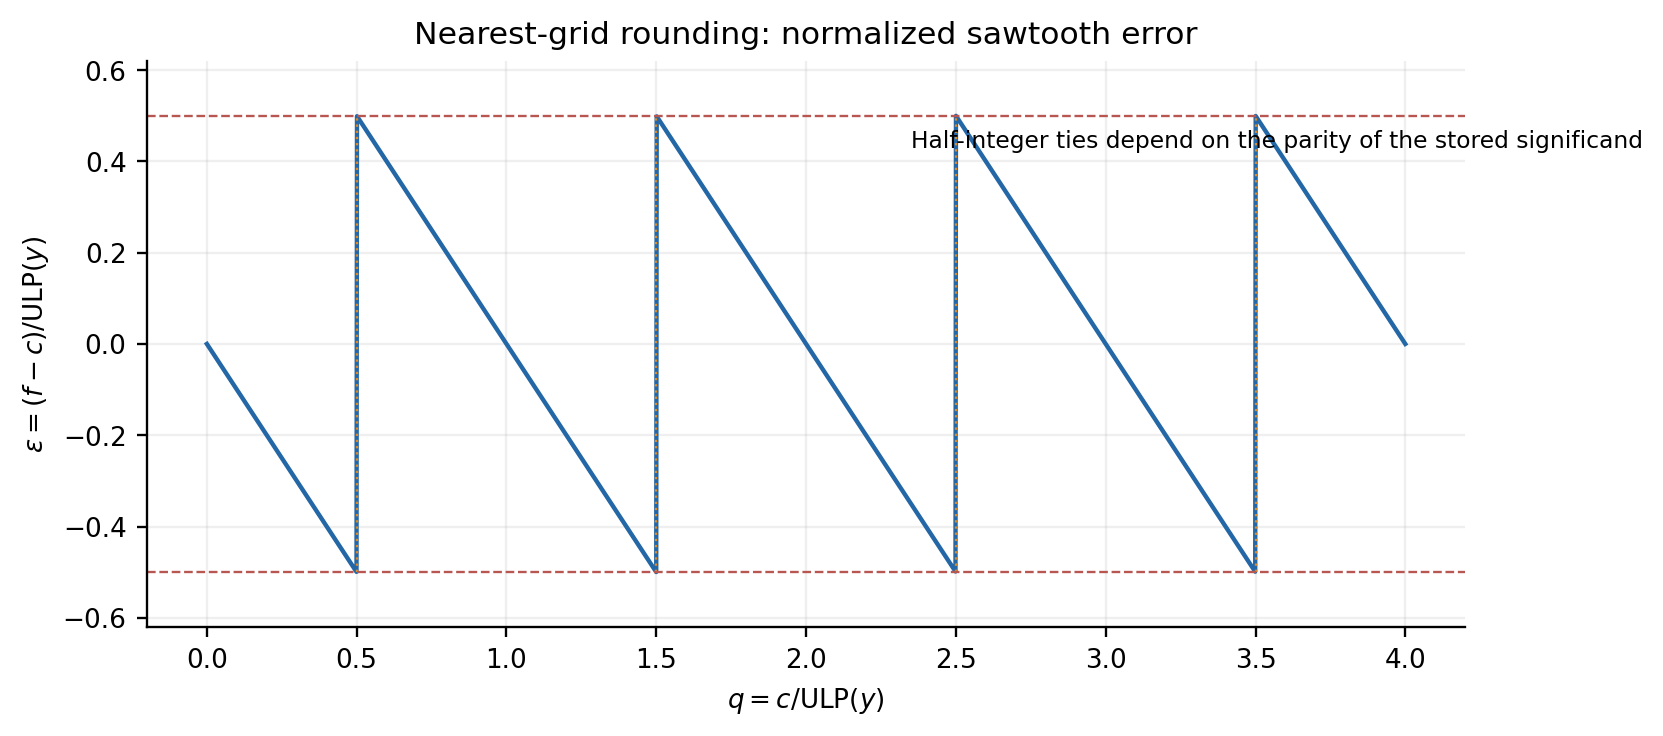
\includegraphics[width=.83\textwidth]{figs/08_ulp_sawtooth.png}
\caption{Theoretical normalized rounding error as a function of the increment measured in ULPs. Values at half-integer ties require the parity rule.}\label{fig:sawtooth}
\end{figure}

\section{Qualifications at binade borders and for \texorpdfstring{$y<c$}{y less than c}}\label{sec:exceptions}
At the upper edge of a binade, $y+c$ may cross into the next binade, where the spacing is $2u$. The fixed-$u$ nearest-grid formula then requires modification. The supplied extended manuscript gives a bound of $|f-c|\le u$ for this crossing case when $y\ge c$, instead of the interior bound $u/2$ \cite{rocha2026bookdraft}.

For $y<c$, the final subtraction need not satisfy Sterbenz's hypotheses, and the same manuscript provides a broader bound $|f-c|\le2\ulp(c)$ with a proof sketch. It reports the stronger empirical observation $|f-c|\le\ulp(c)$ in tested samples, but does not claim to have proved that stronger statement. Neither phenomenon should be hidden by interpreting Equation~\eqref{eq:xthreshold} as a universal exact classification for every $x$.
